\section{Auswertung}

Um die gesuchten Werte und Messgrößen zu bestimmen, ist es nötig im Vorhinein einige wichtige Größen zu bestimmen und festzuhalten.
Die Aktivität des verwendeten Isotops $^{241}\mathrm{Am}$ ist mit \SI{330}{\kilo \becquerel} für das Jahr 1994 gegeben.
Über die Halbwertszeit von Americium kann die Aktivität im Jahr 2024 zu \SI{314.5}{\kilo \becquerel} bestimmt werden. Ein graphischer Verlauf der Aktivität ist
in \autoref{fig:Aktivität} gegeben.
\begin{figure}
    \centering
    \includegraphics[width=1\textwidth]{content/messung/Aktivität.pdf}
    \caption{1.}
    \label{fig:Aktivität}
\end{figure}
Des Weiteren ist es hilfreich im Vorhinein die Teilchenzahl und Dichte für Luft und Gold anzugeben.
Da die Atemluft hauptsächlich aus Stickstoff und Sauerstoff besteht, kann sowohl die mittlere Kernladungszahl als auch die molare Masse und Dichte der Luft 
über die charakteristischen Eigenschaften von Stickstoff und Sauerstoff ausgedrückt werden:
\begin{align*}
Z_{N_2} &= 7 & Z_{O_2} &= 8 & Z_L &= \tfrac{78}{99} Z_{N_2} + \tfrac{21}{99} Z_{O_2} = 7.21 \\
M_{N_2} &= 2 \cdot 14.01 \, \text{g/mol} & M_{O_2} &= 2 \cdot 16.00 \, \text{g/mol} & M_L &= \tfrac{78}{99} M_{N_2} + \tfrac{21}{99} M_{O_2} = 28.86 \, \text{g/mol} \\
\rho_{N_2} &= 1165 \, \text{g/m}^3 & \rho_{O_2} &= 1332 \, \text{g/m}^3 & \rho_L &= \tfrac{78}{99} \rho_{N_2} + \tfrac{21}{99} \rho_{O_2} = 1200 \, \text{g/m}^3 \\
\end{align*}

Die gegebene Dichte und molare Masse von Gold sind:
\begin{align*}
M_G = 196.67 \, \text{g/mol} && \rho_G = 19320 \, \text{g/m}^3 \\
\end{align*}

Hierüber kann die Teilchenzahl von Luft und Gold zu:
\begin{align*}
N_L &= N_A \frac{\rho_L}{M_L} = 250 \cdot 10^{23} \, \text{m}^{-3} \\
N_G &= N_A \frac{\rho_G}{M_G} = 591000 \cdot 10^{23} \, \text{m}^{-3}
\end{align*}
bestimmt werden.

Die druckabhängige Reichweite der $\alpha$-Strahlung ist gegeben über:


\[ \rho = \frac{p}{RT} \qquad R_\alpha \propto p^{-1} \]



Für den Zerfall von $^{241}\text{Am}$ gilt:


\[ ^{241}_{95}\text{Am} \rightarrow ^{237}_{93}\text{Np} + ^4_2\text{He} + E_\alpha \qquad E_\alpha = 5.486 \, \text{MeV} \]



\textbf{Weiß nicht genau, was bei der theoretischen Energieverlustrechnung gemacht wurde. Ist das für Luft?}

\section*{Bestimmung der Dicke der Gold-Folie}

Es werden die gemessenen Maximal-Spannungen in Abhängigkeit des Druckes sowohl mit als auch ohne Gold-Folie im Strahlengang gegen den Druck in der Kammer aufgetragen.
Im Anschluss werden lineare Regressionen durchgeführt. Diese Graphen sind in \autoref{fig:Golddicke} gezeigt.
\begin{figure}
    \centering
    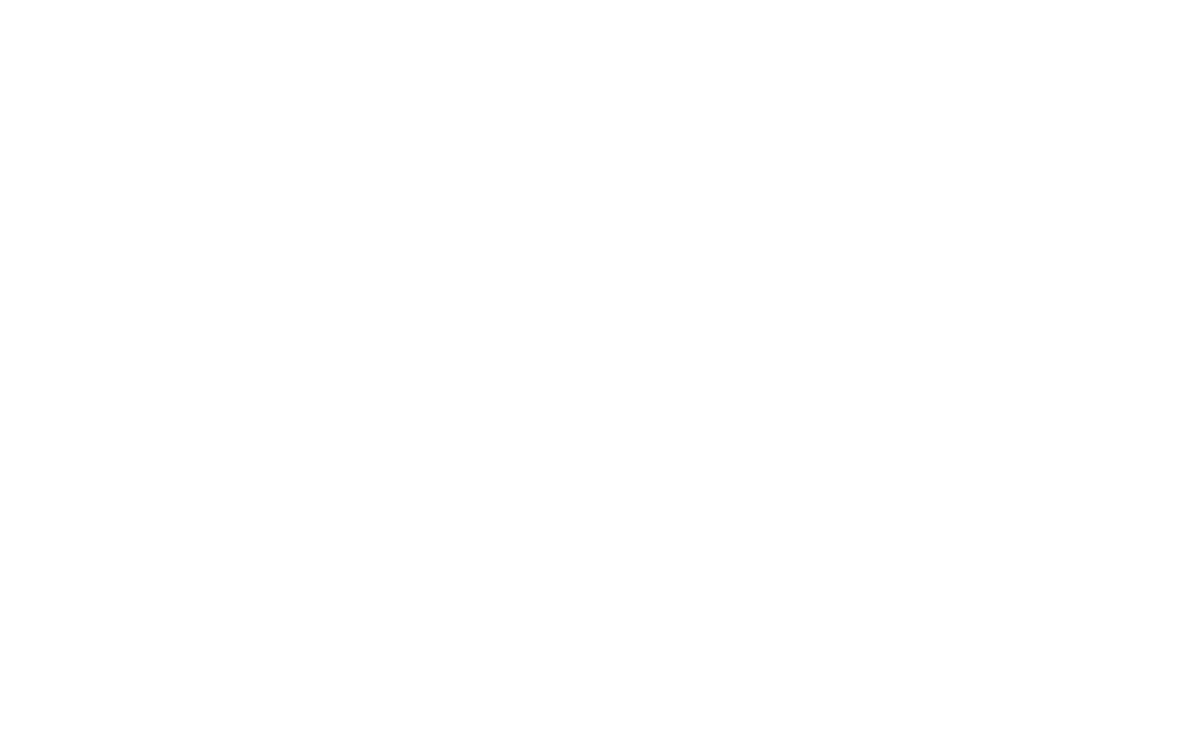
\includegraphics[width=1\textwidth]{content/messung/Golddicke.pdf}
    \caption{1.}
    \label{fig:Golddicke}
\end{figure}
Die Parameter der Geraden $U(p)= ax+b$ ergeben sich zu:
\begin{align*}
    a_{ohne Folie} = -0.0368 \pm 0.0008 \, \frac{\text{V}}{\text{mbar}} & b_{ohne Folie} = 12.10 \pm 0.12 \, \text{V} \\
    a_{mit Folie} = -0.0364 \pm 0.0010 \, \frac{\text{V}}{\text{mbar}} & b_{mit Folie} = 9.65 \pm 0.10 \, \text{V}
\end{align*}


